\begin{center}
\begin{picture}(250,110)
\put(10,105){\vector(1, 0){190}}
\put(10,105){\vector(0, -1){90}}
\put(0,110){$(0,0)$}
\put(205,100){$x$}
\put(10,5){$y$}
\textcolor{blue}{\put(0,40){\line(5,2){200}}}
\put(31,52){\line(-2,5){21}}
\put(20,60){$r$}
\qbezier(15,90)(25,100)(25,105)
\put(16,91){\vector(-1, -1){1}}
\put(25,90){$\theta$}
\end{picture}
\end{center}

%
%\begin{figure}[h]
%\begin{center}
%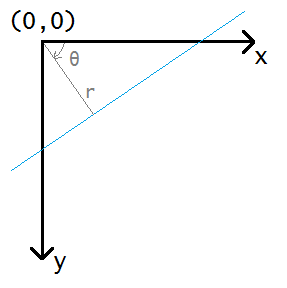
\includegraphics[scale=0.7]{img/lines.png}
%\caption{$(r,\theta)$ parametrization of lines}
%\label{lines_parametrization}
%\end{center}
%\end{figure}